\begin{figure}[htbp]

\begin{center}
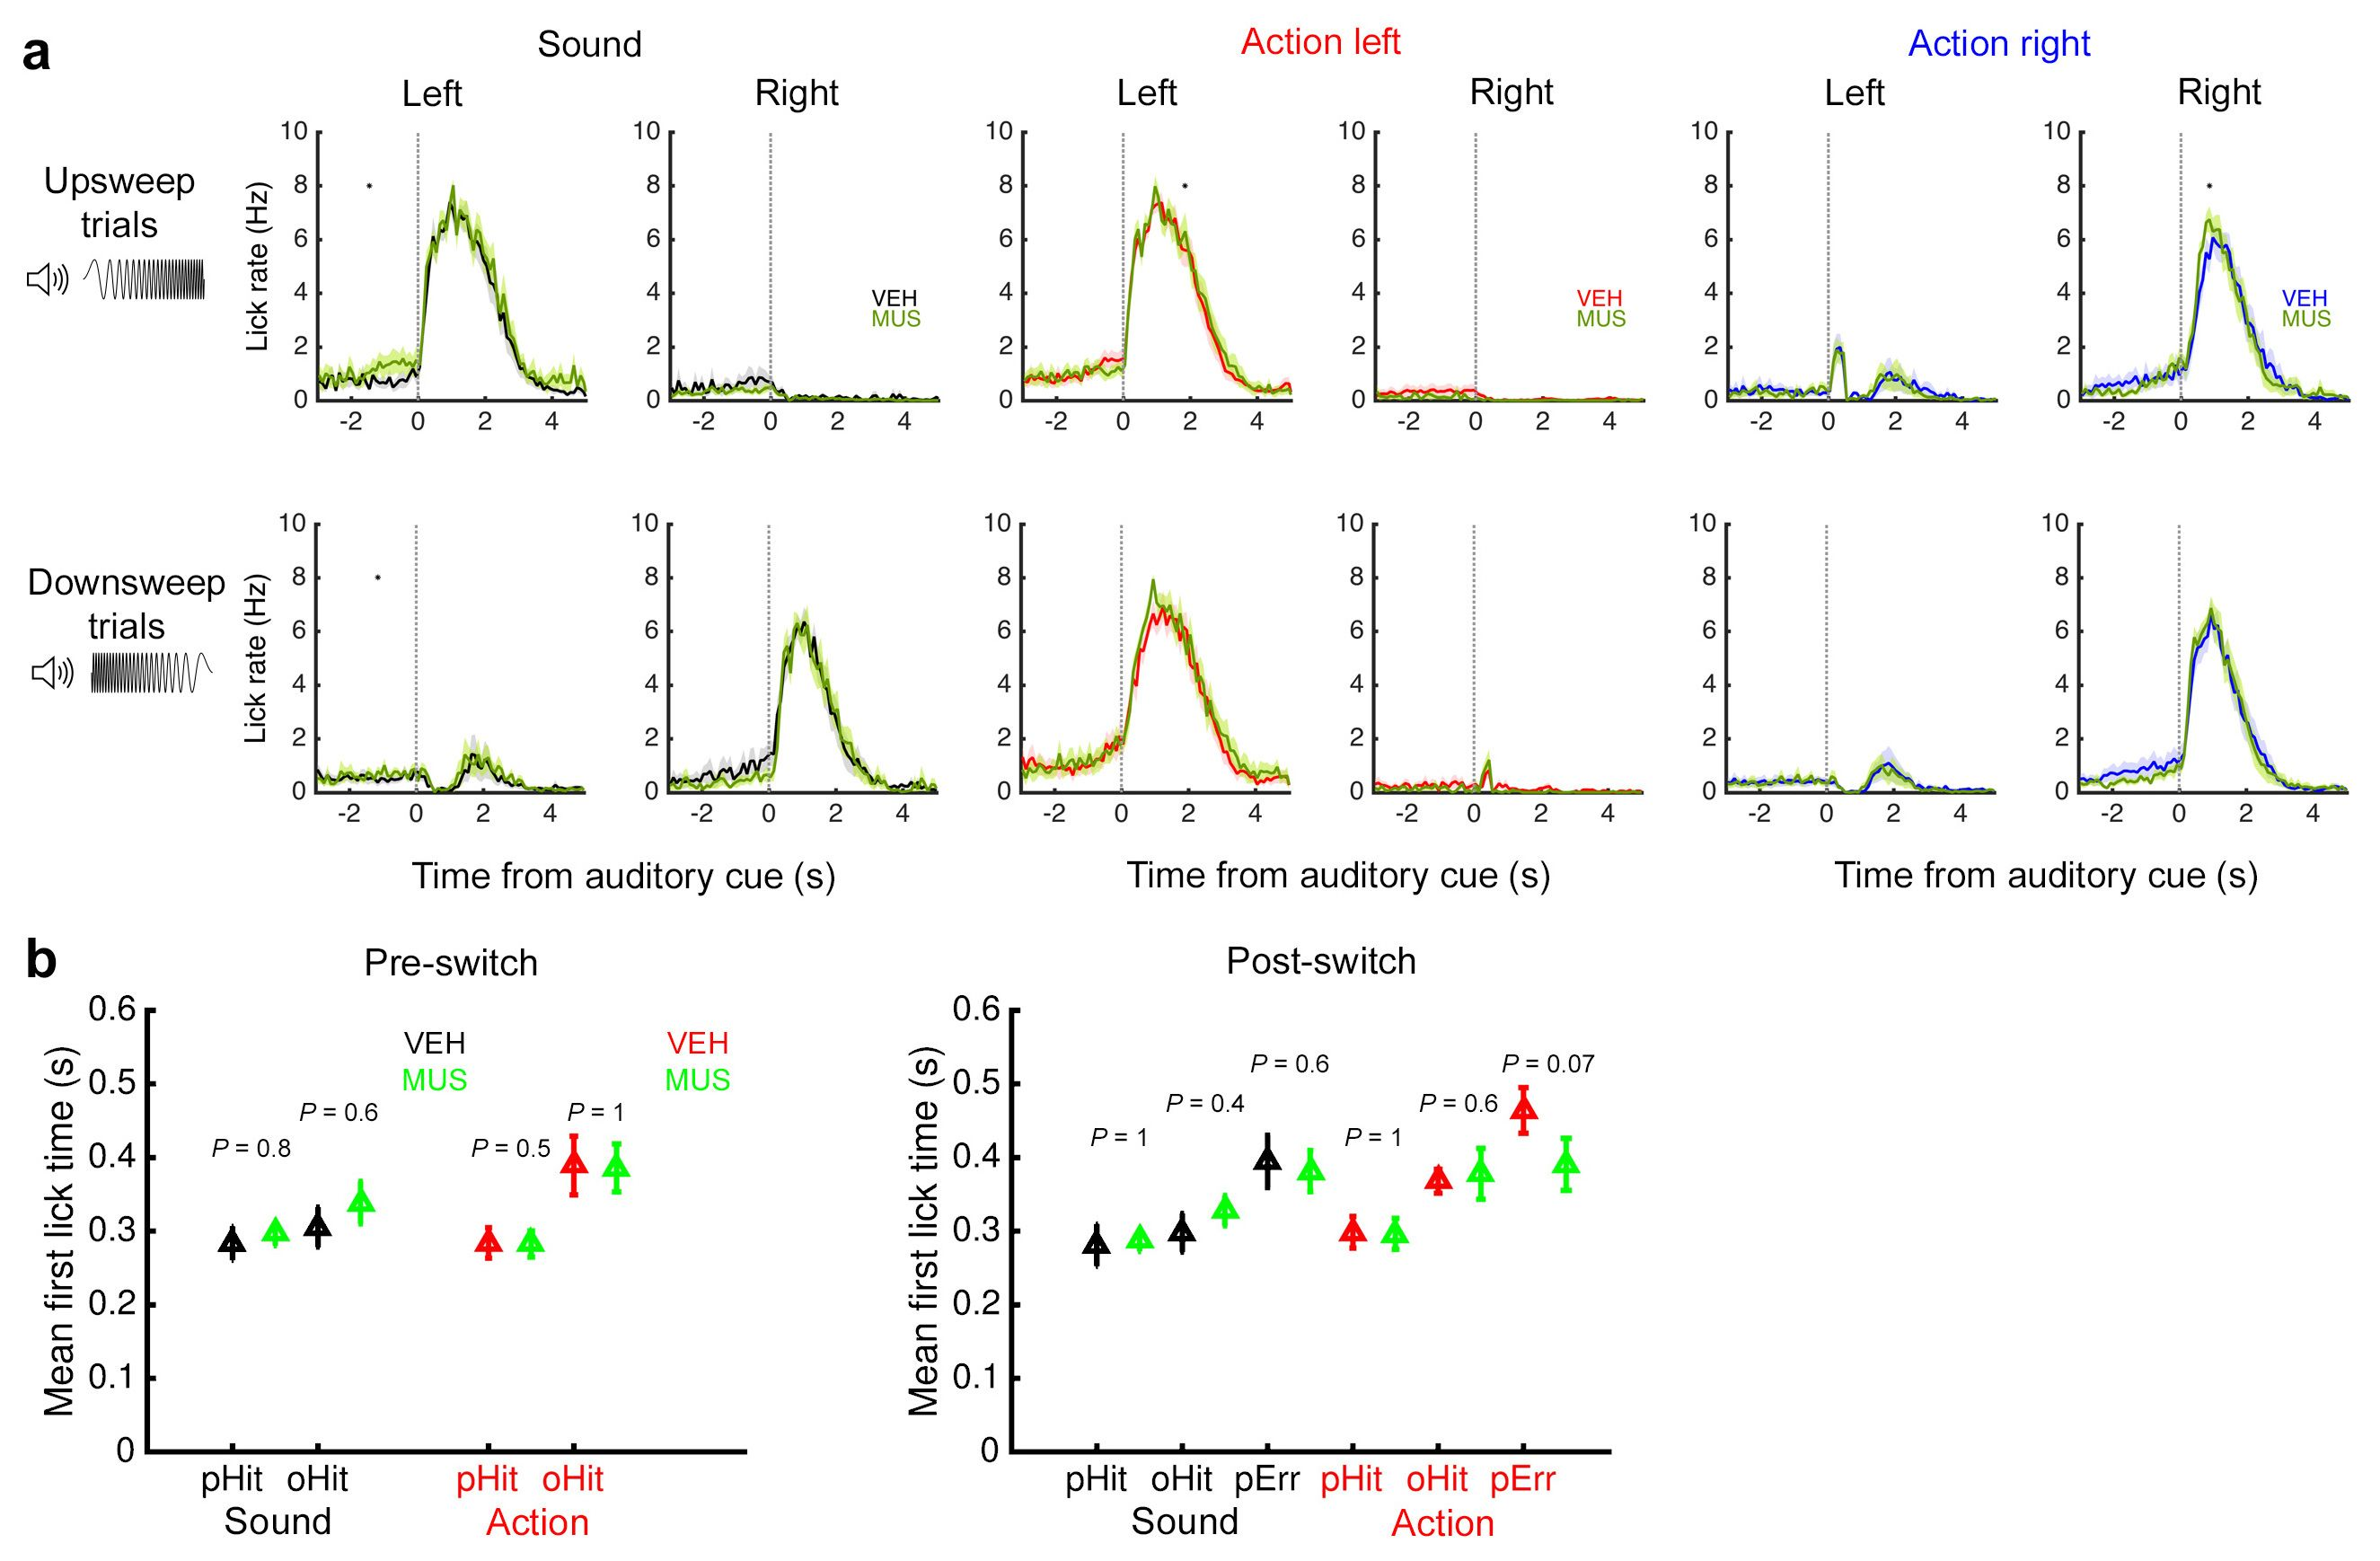
\includegraphics[width=\textwidth]{Figures/Chapter3/NN_figS5.jpg} 
\end{center}

\caption[M2 inactivation did not affect mean lick rate or response time]
{Bilateral inactivation of M2 had no effect on mean lick rate or response time.
(a) Same analysis as Fig. \ref{fig:NN_fig1}e using data from saline- (black, red, blue) and muscimol-injected mice (overlaid in green). Lick rates in each rule-sensory-motor combination were compared between saline and muscimol conditions for each 0.1 s bin. The bars at the top of the panels denote significant differences ($p<0.01$, t-test; only 4 bins had significant difference by this measure, and none were consecutive bins). Data presented as $\mathit{mean}\pm\mathit{SEM}$ (b) Same analysis as Supplementary Fig. \ref{fig:NN_figS2}c, using data from the saline- (black, red) and muscimol-injected (green) mice. The Wilcoxon signed-rank test was used to assess differences between saline and muscimol conditions. $N = 11$ mice.}

\label{fig:NN_figS5}
\end{figure}